\documentclass{article}
\usepackage{spconf,amsmath,amssymb,graphicx,booktabs,url}
% Verified values generated from the paused snapshots.
\newcommand{\BaseBest}{0.025080}
\newcommand{\BaseEnd}{0.025618}
\newcommand{\BridgeBest}{0.024445}
\newcommand{\BridgeEnd}{0.028603}
\newcommand{\BridgeBestGain}{2.53}
\newcommand{\BridgeEndHarm}{11.65}
\newcommand{\SensorBestGain}{1.36}
\newcommand{\SensorEndHarm}{1.21}
\newcommand{\BridgeSSIM}{0.93509}
\newcommand{\BaseSSIM}{0.93878}
\newcommand{\BridgePatchWins}{63}
\newcommand{\BridgeDiff}{0.635}
\newcommand{\BridgeLower}{-0.005}
\newcommand{\BridgeUpper}{1.256}
\newcommand{\BridgeLow}{+7.71}
\newcommand{\BridgeMid}{+5.39}
\newcommand{\BridgeHigh}{-5.19}
\newcommand{\BridgeExtraParams}{9,223}

\newcommand{\StageResultRows}{%
Base & 0.025618 & 32 & 0.025080 & \textemdash & 0.93878 & 0.08987 & 1.0701 & 0.82951 \\
I02 & 0.028603 & 9 & 0.024445 & +2.53 & 0.93509 & 0.08641 & 0.9715 & 0.82545 \\
I01 & 0.025929 & 22 & 0.024740 & +1.36 & 0.94123 & 0.08470 & 1.0037 & 0.82605 \\
I06 & 0.026038 & 32 & 0.025230 & -0.60 & 0.93716 & 0.08892 & 1.0811 & 0.82428 \\
I03 & 0.025477 & 38 & 0.025350 & -1.07 & 0.93865 & 0.09061 & 1.0832 & 0.82415 \\
I05 & 0.026412 & 24 & 0.025371 & -1.16 & 0.93863 & 0.08789 & 1.0560 & 0.82452 \\
I07 & 0.026729 & 18 & 0.025494 & -1.65 & 0.93504 & 0.08966 & 1.0870 & 0.82551 \\
I13 & 0.026042 & 32 & 0.025517 & -1.74 & 0.93904 & 0.08903 & 1.0535 & 0.81914 \\
}

\graphicspath{{figures/}}
\newcommand{\obs}{\mathcal{O}}
\newcommand{\target}{F^\star}
\title{A DUAL-ANCHOR DIFFUSION BRIDGE FOR ONE-STEP REMOTE SENSING SPATIOTEMPORAL FUSION}
\name{Anonymous Authors}
\address{Interim manuscript, 22 November 2026}

\begin{document}
\ninept
\maketitle

\begin{abstract}
One-step spatiotemporal fusion reconstructs a fine-resolution image from coarse observations and fine references with a single denoising call. We study how the initial noisy state affects this reconstruction. A dual-anchor diffusion bridge centers the state on a date-weighted, observation-derived prior and predicts a spatial noise scale from the same inputs. On the Lower Gwydir Catchment (LGC) development split, the bridge reduces mean patch RMSE from \BaseBest{} to \BridgeBest{} (\BridgeBestGain\%) at the checkpoints selected by validation RMSE. At the shared 40-epoch endpoint, RMSE instead rises from \BaseEnd{} to \BridgeEnd{}. Across coarse-deviation tertiles, the selected bridge helps on patches closer to the coarse anchor blend and loses accuracy in the highest tertile. The observations come from one training seed and one validation date. They identify checkpoint selection and coarse temporal deviation as conditions that matter when evaluating the bridge.
\end{abstract}

\begin{keywords}
spatiotemporal fusion, remote sensing, diffusion bridge, dual anchors, validation trajectory
\end{keywords}

\begin{figure*}[!t]
\centering
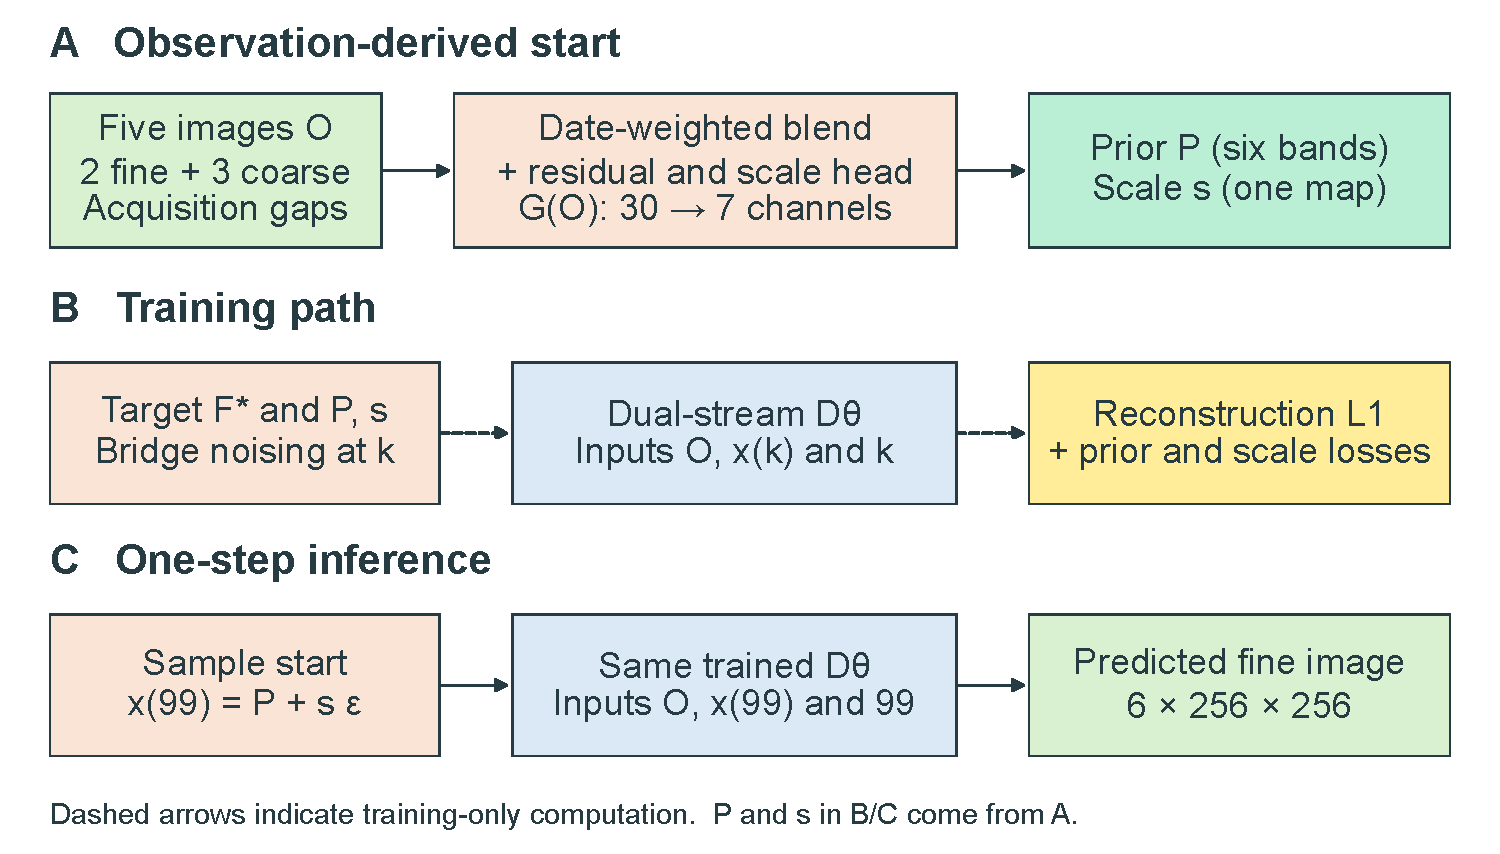
\includegraphics[width=.91\textwidth]{bridge.pdf}
\caption{The bridge derives a prior $P$ and scale $s$ from the five observations. The training-only target $\target$ enters the forward state and losses in panel B. At inference the network predicts from $P+s\varepsilon$ with one call. Labels $x(k)$ and $x(99)$ denote $X_k$ and $X_{99}$.}
\label{fig:bridge}
\end{figure*}

\section{Introduction}
Satellite observations that resolve fine spatial structure often have limited temporal coverage. A dual-anchor fusion model uses two fine reference images and three coarse observations to estimate the missing fine image at an intermediate date. The coarse observation records target-date change at its native scale. Fine references locate earlier and later structures whose positions and appearance may differ at the target date.

Conditional diffusion models such as STFDiff incorporate these observations into denoising~\cite{huang2024stfdiff}. A single denoising call compresses the reconstruction budget~\cite{song2021ddim}. In the local one-step baseline studied here, the denoiser starts from standard Gaussian noise, while the two available fine anchors enter through conditioning. We ask whether an observation-derived starting distribution improves validation accuracy under the same number of denoiser evaluations, and whether any gain persists at a shared training endpoint.

We build a dual-anchor diffusion bridge in a common STFDiff-based backbone. The starting state combines a date-weighted fine-image blend, a learned residual, and a learned noise scale (Fig.~\ref{fig:bridge}). We evaluate eight completed runs under one 40-epoch budget, report both checkpoint selection rules, and examine paired patch errors across levels of coarse temporal deviation. A separate sensor-operator variant tests an intervention after denoising.

\section{Related work}
STFDiff learns a conditional distribution of fine images from reference observations~\cite{huang2024stfdiff}. SA-STF applies residual diffusion with temporal feature alignment and semantic-adaptive fusion~\cite{zhang2026sastf}. Recent restoration work guides diffusion bridges with spatial uncertainty~\cite{tu2026udbm}. In remote sensing, WPFM-STF transports a learned temporal prior to the target through flow matching with wavelet constraints~\cite{hu2026wpfm}. Our comparison keeps the same five observations and denoising backbone. It evaluates a date-weighted dual-anchor prior and Gaussian scale in the forward noising process and one-step starting state.

\section{Method}
\subsection{Observation protocol}
Let $\obs=(F_-,F_+,C_-,C_0,C_+)$ denote earlier and later fine observations, their co-registered coarse observations, and the target-date coarse observation $C_0$. Images are on a common $256\times256$ grid with six bands. The model uses values in $[-1,1]$ and evaluates predictions in reflectance space. Denote the unavailable target fine image by $\target$. It enters the training noising process and losses, and it serves as the evaluation reference.

\subsection{Dual-anchor starting distribution}
Let $\Delta_-$ and $\Delta_+$ be the day gaps from the earlier anchor to the target and from the target to the later anchor. The interpolation weight is $w=\Delta_-/(\Delta_-+\Delta_+)$. A head $G$ maps the concatenated 30 image channels to seven maps $q=G(\obs)$. It uses a $3\times3$ convolution, a depthwise $3\times3$ convolution, and a $1\times1$ projection with width 32 in the first two layers. The bounded residual and scale yield
\begin{align}
P&=(1-w)F_-+wF_++0.2\tanh(q_{1:6}),\\
s&=0.05+0.45\,\mathrm{sigmoid}(q_7).
\end{align}
$P$ has six bands and each pixel of $s$ is shared across the six bands. The date gaps set the interpolation weights. The head obtains its inputs from the five images.

With the 100-level cosine schedule $\bar\alpha_k$, training constructs the perturbed image
\begin{equation}
X_k=P+\sqrt{\bar\alpha_k}(\target-P)
       +\sqrt{1-\bar\alpha_k}\,s\varepsilon,\quad
\varepsilon\sim\mathcal{N}(0,I),
\label{eq:bridge}
\end{equation}
where $k\in\{0,\ldots,99\}$. The dual-stream predictor $D_\theta$ encodes $\obs$ and $X_k$ separately, then predicts the fine image with residual features and noise-time conditioning. The reconstruction is clipped to $[-1,1]$. Its loss is $\operatorname{MAE}(\widehat{F},\target)+\mathcal{L}_{P,s}$, where
\begin{align}
\mathcal{L}_{P,s}={}&0.1\left\langle |P-\target|\right\rangle\\
&+0.005\left\langle
\frac{(P-\target)^2}{s^2+10^{-6}}+2\log s\right\rangle .
\end{align}
Angle brackets average pixels and bands. The last term weights residuals by the predicted scale. It trains a noise map whose calibration requires independent evaluation.

For inference, the initial state is $X_{99}=P+s\varepsilon$. The sampler calls $D_\theta(\obs,X_{99},99)$ once and returns its clipped prediction. With $P=0$ and $s=1$, the base configuration recovers the Gaussian start and omits the auxiliary loss. Both settings use one denoiser evaluation. The bridge adds \BridgeExtraParams{} parameters to the base of 7,488,966 and makes one additional head evaluation.

\subsection{Sensor-operator comparison}
I01 keeps the Gaussian start and applies two data consistency updates after denoising. A learned linear operator $S$ consists of a normalized $5\times5$ blur per band and a row-normalized $6\times6$ spectral mix. A smoothed, date-weighted blend of the anchor residuals $C_\pm-S(F_\pm)$ estimates bias $b$. Each update is
\begin{equation}
Y_{j+1}=Y_j-\lambda S^\top(S(Y_j)+b-C_0),\quad j=0,1 .
\end{equation}
The step $\lambda$ is learned and bounded by a sigmoid. Training also penalizes anchor observation residuals. This branch represents a separate mechanism following the common backbone.

\begin{table*}[!t]
\centering
\caption{LGC development results for 120 patches, one training seed (42), and one denoiser evaluation. Epoch 40 RMSE uses the recorded common endpoint. Best RMSE and other metrics use each method's minimum-validation-RMSE checkpoint. A positive gain is a reduction relative to the paired base best checkpoint.}
\label{tab:main}
\setlength{\tabcolsep}{5pt}
\begin{tabular}{lrrrrrrrr}
\toprule
Method & Epoch 40 RMSE $\downarrow$ & Best epoch & Best RMSE $\downarrow$ & Gain (\%) &
SSIM $\uparrow$ & SAM $\downarrow$ & ERGAS $\downarrow$ & CC $\uparrow$ \\
\midrule
\StageResultRows
\bottomrule
\end{tabular}
\end{table*}

\begin{figure*}[!t]
\centering
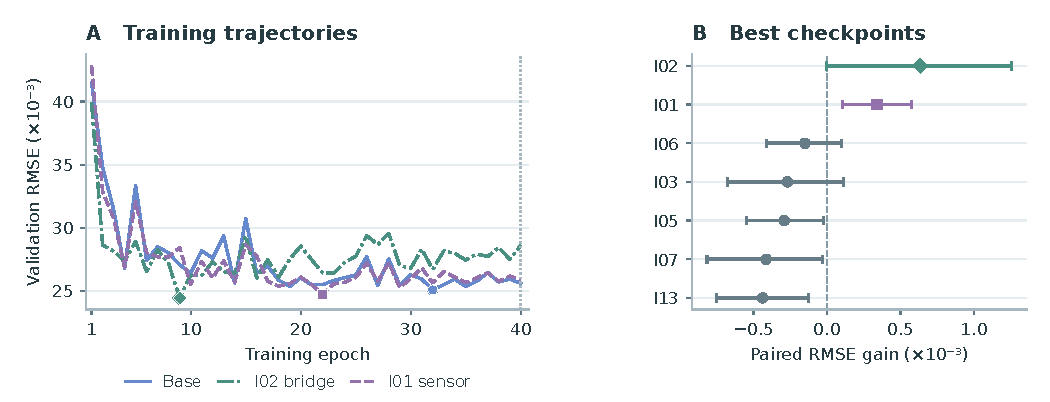
\includegraphics[width=\textwidth]{validation_dynamics_en.pdf}
\caption{A. Validation trajectories with markers at selected checkpoints and a dotted line at the shared epoch 40. B. Best-checkpoint RMSE gains, defined as base minus variant. Dots are paired means. Intervals are 2.5th--97.5th percentiles from 10,000 resamples of 30 fixed, nonoverlapping $2\times2$ patch blocks within the validation scene.}
\label{fig:curves}
\end{figure*}

\section{Experiments}
\subsection{Data, training, and evaluation}
The LGC image series~\cite{emelyanova2013blending} supplies the two-resolution observations. Our training split contains 1,200 patches from ten triples. Validation uses 120 nonoverlapping patches from one triple (14 February, 2 March, and 3 April 2005). The target fine date is absent from the training inputs and targets. These are development data on a historically used scene. We froze the split and analyzed every completed from-scratch run at the pause, comprising the baseline and seven variants at seed 42.

Each run uses Adam for 40 epochs and 600 optimizer updates per epoch, a peak learning rate of $2\times10^{-4}$, 50-step warm-up, cosine decay to one tenth of the peak, and clipping of the gradient norm to 1. A microbatch of one and accumulation of two hold effective batch size fixed. We use paired sample ordering, initialization of the shared backbone, and base-noise draws within the seed block.

The validation RMSE averages patch-level reflectance RMSE over the 120 patches and three fixed per-patch noise realizations. At the common epoch 40, we report the saved validation RMSE. For each method's best checkpoint, we use the minimum over the 40 saved validations and its exported metrics, including SSIM, spectral angle (SAM, radians), ERGAS (ratio $1/16$), and correlation coefficient (CC). Paired patch analyses first average the three noise realizations per patch.

\subsection{Training endpoint and selected checkpoint}
Table~\ref{tab:main} shows that I02 achieved the lowest best-checkpoint RMSE, from \BaseBest{} to \BridgeBest{}, while I01 lowered error by \SensorBestGain\%. I02 improved SAM and ERGAS with a small decline in SSIM and CC. At epoch 40, I02 and I01 had higher RMSE by \BridgeEndHarm\% and \SensorEndHarm\%, respectively. I03 is the only variant in this set with lower RMSE than base at epoch 40.

I02 reached its minimum at epoch 9. The base reached its minimum at epoch 32. The complete trajectories in Fig.~\ref{fig:curves} retain the later error increase. In the earlier six-epoch warm-start screen, none of the 14 variants crossed the improvement gate against the stronger original control. The different ordering under from-scratch training motivates treating both the training recipe and checkpoint rule as parts of the comparison.

\subsection{Where bridge gains occur}
At the selected checkpoints, I02 reduced error on \BridgePatchWins{} of 120 patches. Its mean paired gain of $\BridgeDiff\times10^{-3}$ has a descriptive block-resampling interval of $[\BridgeLower,\BridgeUpper]\times10^{-3}$, which spans zero. The interval describes spatial variation for these fitted runs. It leaves training-seed and date variability open.

To examine patch heterogeneity, we rank the patches by the mean absolute deviation between $C_0$ and $(1-w)C_-+wC_+$, calculated on the observed coarse images in reflectance space. Each tertile contains 40 patches. Across increasing tertiles, the relative reductions are \BridgeLow\%, \BridgeMid\%, and \BridgeHigh\% (Fig.~\ref{fig:strata}). Thus the mean accuracy gain is concentrated where the target coarse observation is closer to the interpolated anchors.

\begin{figure}[!t]
\centering
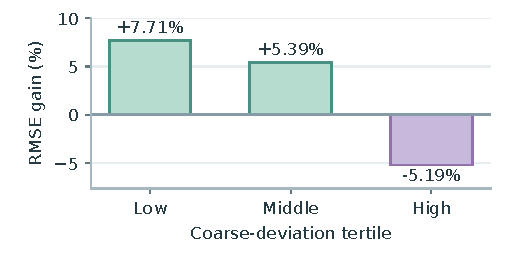
\includegraphics[width=\columnwidth]{coarse_strata_en.pdf}
\caption{I02 relative RMSE gain over base at their selected checkpoints within each observed coarse-deviation tertile (40 patches each). These post hoc groups quantify compatibility with the coarse anchor blend.}
\label{fig:strata}
\end{figure}

\clearpage
\raggedbottom
\section{Discussion and conclusion}
The bridge yielded a lower early validation minimum and a higher error at the common endpoint. This makes the checkpoint rule consequential for claims about one-step fusion. The higher-deviation patches suggest where an interpolated prior may be less useful. Coarse deviation also reflects observation differences, so this analysis cannot identify the influence of true land-cover change. The prior, scale, and auxiliary losses change together in I02, and their separate effects remain open.

I01 improves its selected-checkpoint RMSE by enforcing observation consistency after denoising. A fair comparison of both interventions uses their learning curves and a shared endpoint. Additional seeds and independent scenes in LGC and the Coleambally Irrigation Area (CIA) can test stability and transfer. External comparison requires a common protocol. The SA-STF authors' training split includes our 2 March 2005 validation date~\cite{zhang2026sastf}.

\textbf{Reproducibility.} The stage archive provides the frozen manifest, run records, and code for the tables and figures.

\par\vfill\newpage
\bibliographystyle{IEEEbib}
\bibliography{refs}
\end{document}
